\documentclass{article}

\usepackage{graphicx}
\usepackage{subcaption}
\usepackage{geometry}
%\geometry{total={8in,11in},left=0in, top=0in}

\begin{document}


\begin{figure}[h!]
\centering
\begin{subfigure}[b]{0.45\linewidth}
  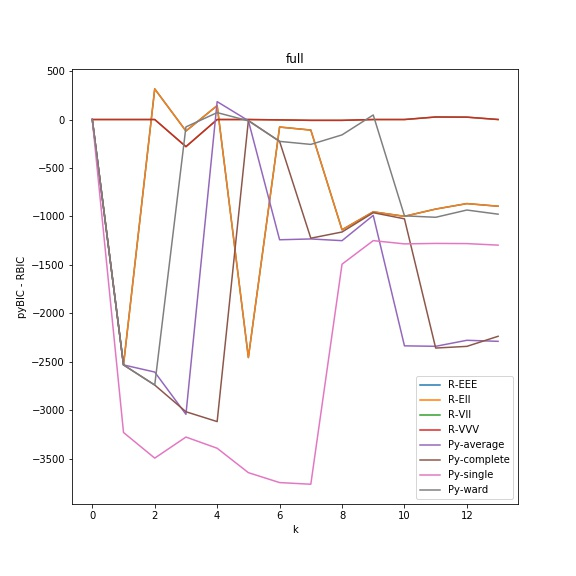
\includegraphics[width=\linewidth]{full.jpg}
\end{subfigure}
\begin{subfigure}[b]{0.45\linewidth}
  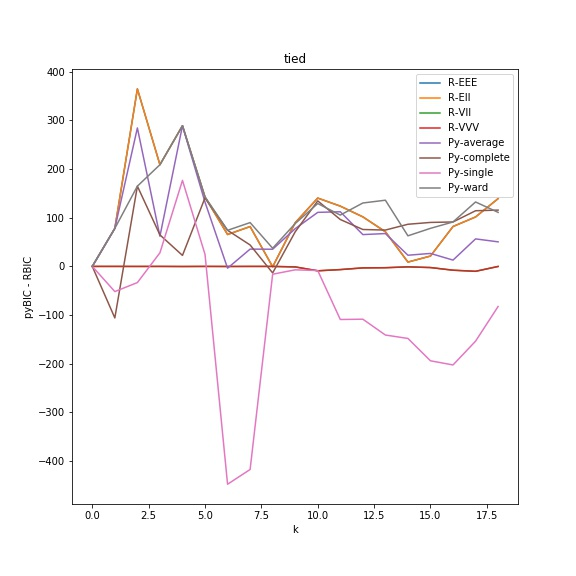
\includegraphics[width=\linewidth]{tied.jpg}
\end{subfigure} 

\begin{subfigure}[b]{0.45\linewidth}
  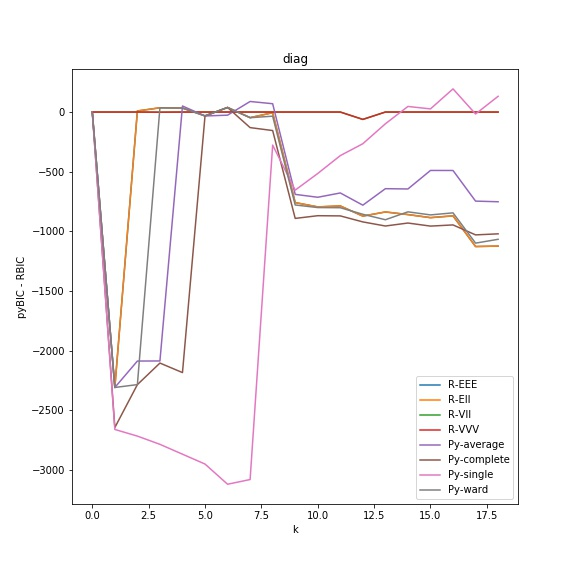
\includegraphics[width=\linewidth]{diag.jpg}
\end{subfigure}
\begin{subfigure}[b]{0.45\linewidth}
  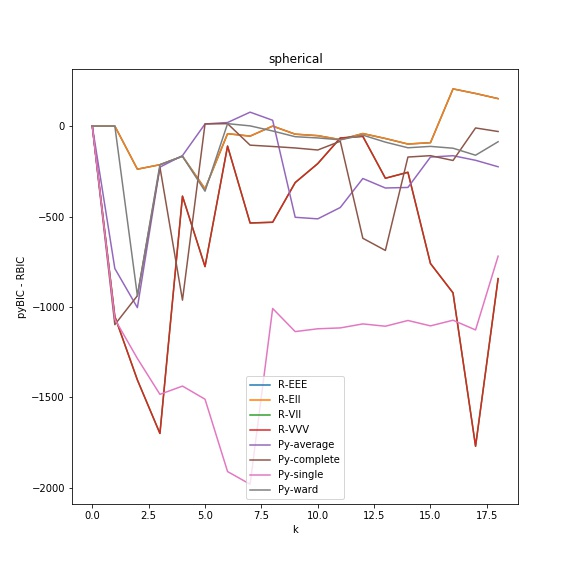
\includegraphics[width=\linewidth]{spherical.jpg}
\end{subfigure} 
\end{figure}

\begin{itemize}
\item The purpose of these figures is to use BIC to compare the performance of the EM algorithm between R's mclust and Python's GaussianMixture. 
\item I did this by saving the results of different methods of hierarchical agglomeration, then using these as initializations of the EM algorithms. 
\item Each line in the plots above corresponds to a different hierarchical agglomeration method (R's EEE, EII, VII,VVV modes and Python's average, complete, single, and ward's linkages on euclidean distance = 8 total agglomeration methods)
\item Each plot corresponds to an EM mode that is implemented in BOTH python and mclust. For example 'full' mode in GaussianMixture and 'VVV' mode in mclust are \textit{theoretically} equivalent and they are found in the plot titled 'full', the other pairs are: 'tied'='EEE', 'diag'='VVI', and 'spherical'='VII
\item The y axis in each plot is python's BIC minus R's BIC. So, negative values indicate that R did better, according to BIC
\end{itemize}

\end{document}